\section{Two-way tables}\label{sec:mosaic-twoway}
The mosaic display 
\citep{Friendly:92b,Friendly:94a,Friendly:97,HartiganKleiner:81,HartiganKleiner:84}
is like a grouped barchart,
where the widths of the bars show the relative frequencies of one
variable, and heights of the sections in each bar show the
relative frequencies of the second variable as shown in \figref{fig:mosaic31}.
% Additional variables can be displayed by dividing 
The construction of the mosaic display, and what it reveals,
are most easily understood for two-way tables.

\begin{Example}[haireye2a]{Hair color and eye color}
Consider the data in \tabref{tab:hairdat},
showing the relation between hair color and eye color among students
in a statistics course.
\begin{figure}[htb]
  \centering
  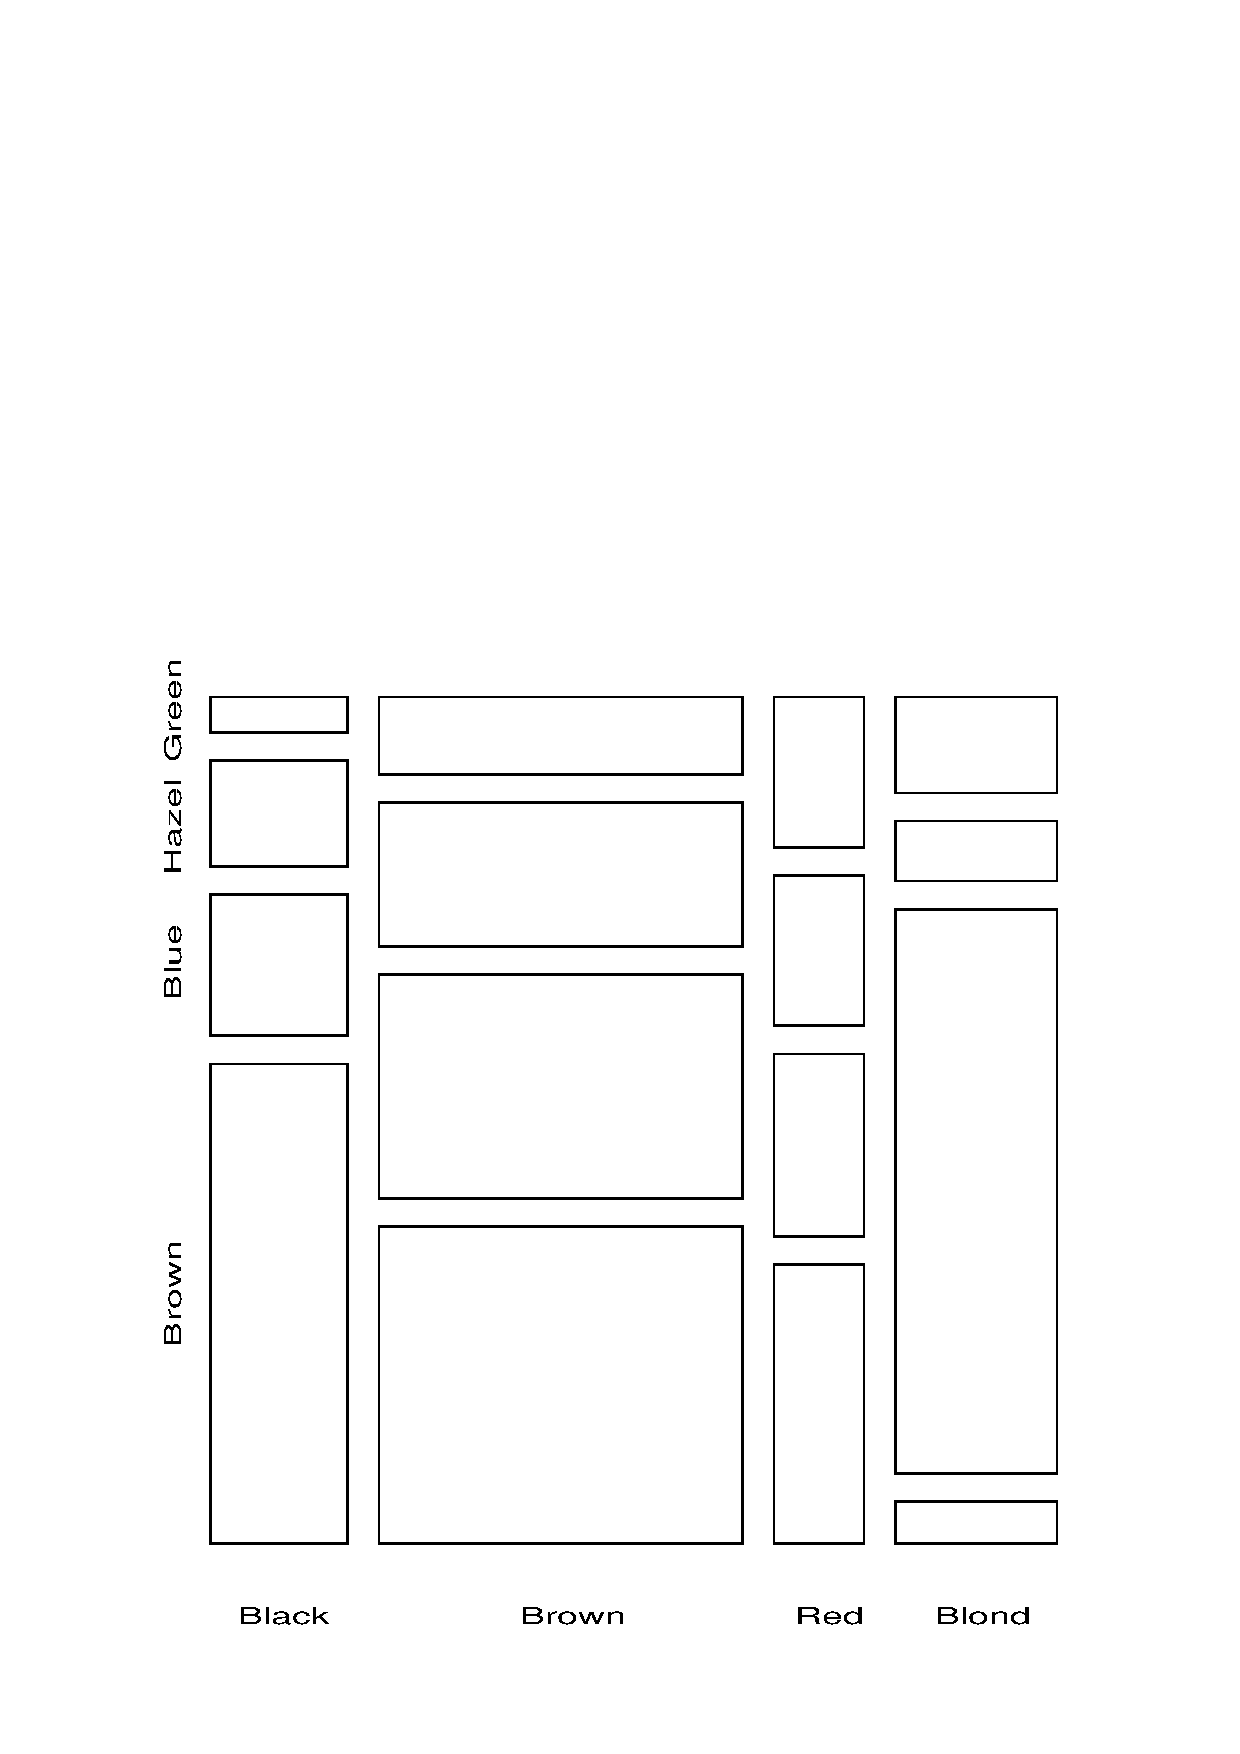
\includegraphics[scale=.6]{ch4/fig/mosaic31}
  \caption[Basic mosaic display for hair color and eye color data]{Basic mosaic display for hair color and eye color data.  The area of each
  rectangle is proportional to the observed frequency in that cell.}%
  \label{fig:mosaic31}
\end{figure}
For such a two-way table, the mosaic display is constructed
by first dividing a unit square in proportion to the marginal
totals of one variable, say, Hair color.

For these data, the marginal frequencies and proportions are:

\begin{minipage}{\linewidth} 
\begin{verbatim} 
              Black      Brown      Red    Blond    TOTAL
Frequencies    108       286        71      127      592
Proportions   0.1824    0.4831    0.1199   0.2145   1.000
\end{verbatim}
\end{minipage}


These can be shown as the mosaic for the first variable (hair color),
as in \figref{fig:mosaic32}.
The rectangular tiles are shaded to show the residuals (deviations)
from a particular model, as follows:
\begin{figure}[htb]
  \centering
  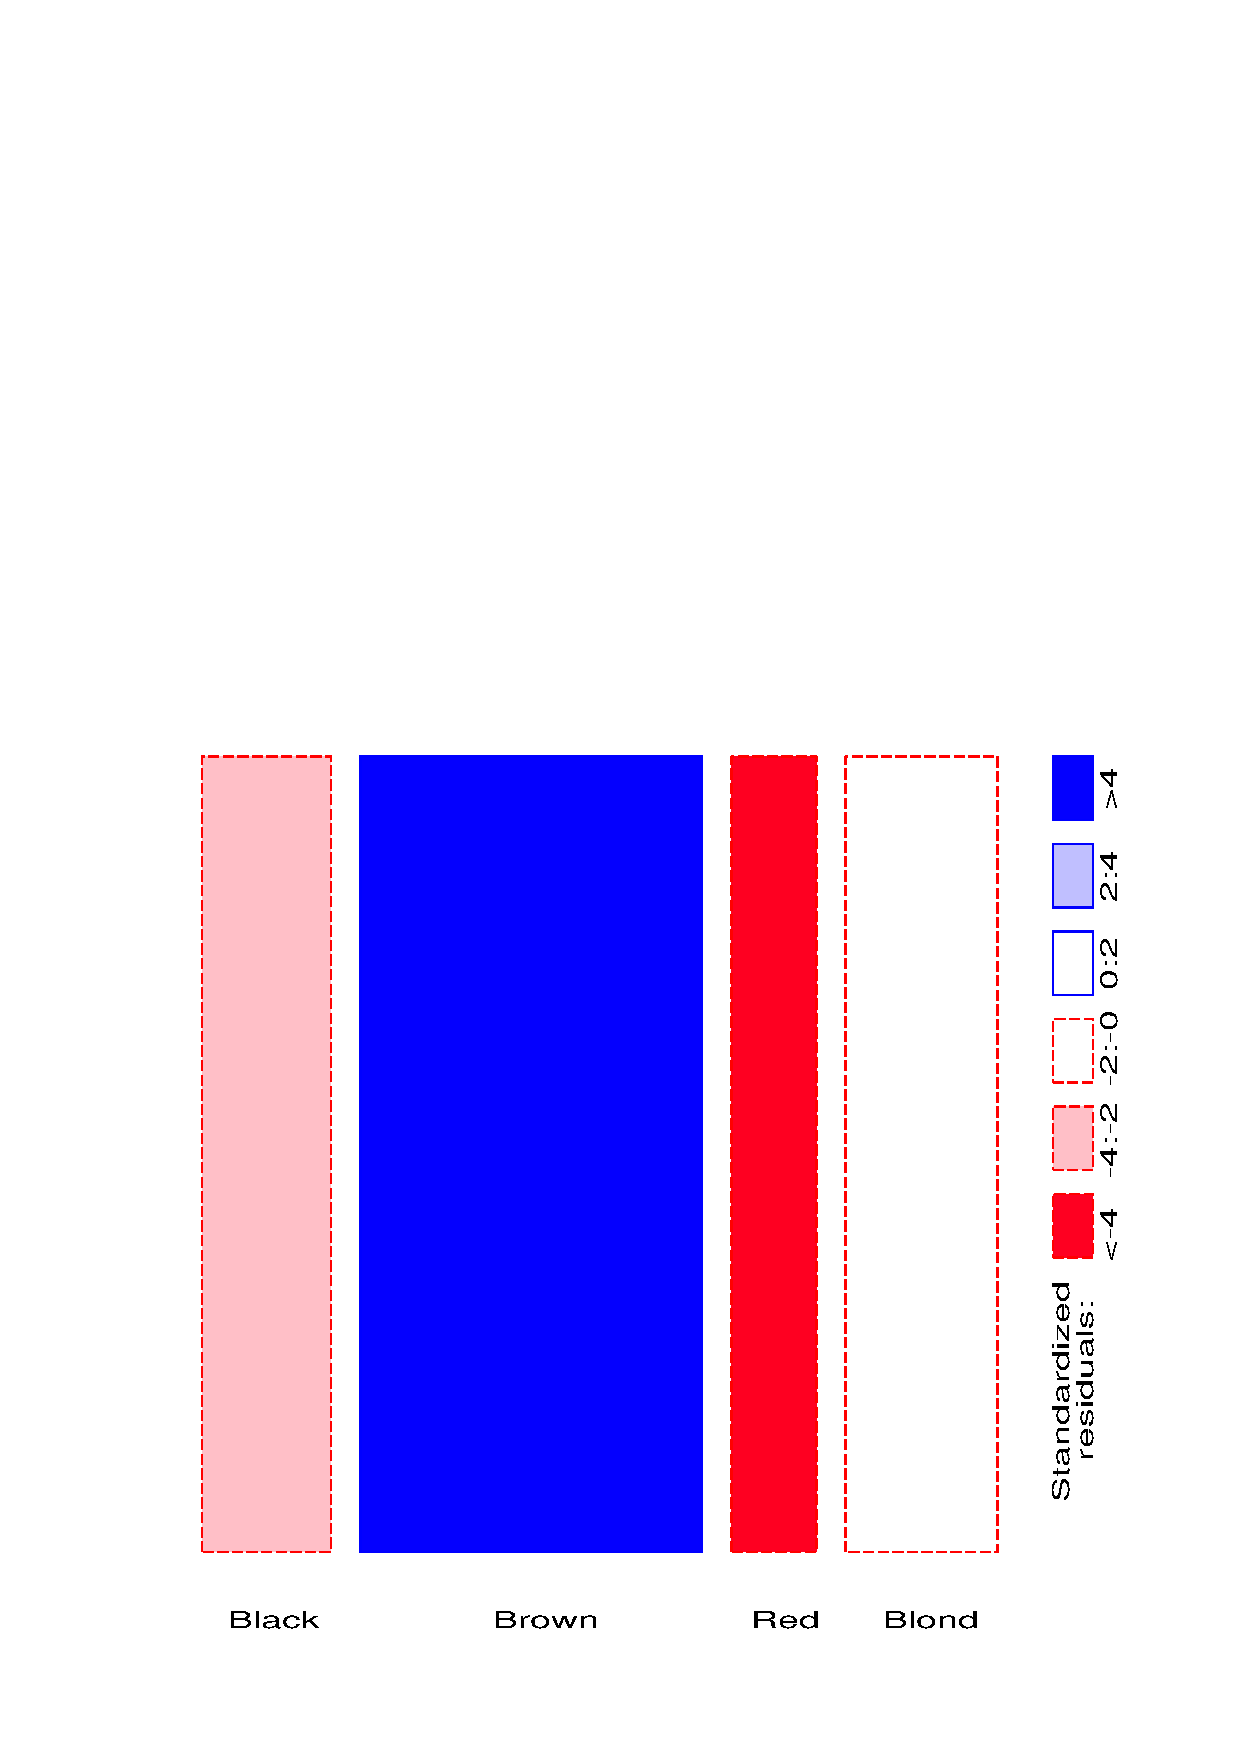
\includegraphics[scale=.6]{ch4/fig/mosaic32}
  \caption{First step in the mosaic display}%
  \label{fig:mosaic32}
\end{figure}

\begin{itemize}
\item The one-way table of marginal totals can be fit to a model, in this
case, the model that all hair colors are equally probable.  This model
has expected frequencies $m_i = 592/4$:
\begin{verbatim} 
               Fitted frequencies
       Black      Brown      Red    Blond
       148.00    148.00    148.00   148.00
\end{verbatim}
\item The Pearson residuals from this model, $d_i = ( n_i - m_i ) / \sqrt{m_i}$, are:
\begin{verbatim} 
         Standardized Pearson residuals
       Black    Brown      Red    Blond
       -3.29    11.34    -6.33    -1.73
\end{verbatim}
and these values are shown by color and shading as shown in the legend.
The high positive value for Brown hair indicates that people
with brown hair are much more frequent in this sample than 
the Equiprobability model would predict.
\end{itemize}

Next, the rectangle for each Hair color is subdivided in proportion
to the relative (conditional) frequencies of the second variable --
Eye color, giving the following conditional proportions:
\begin{verbatim} 
                     Marginal proportions
                Brown     Blue    Hazel    Green   TOTAL

      Black    0.6296   0.1852   0.1389   0.0463    1.0
      Brown    0.4161   0.2937   0.1888   0.1014    1.0
      Red      0.3662   0.2394   0.1972   0.1972    1.0
      Blond    0.0551   0.7402   0.0787   0.1260    1.0
\end{verbatim}
The proportions in each row determine the heights of the tiles in the second mosaic display in \figref{fig:mosaic33}.
\begin{figure}[htb]
  \centering
  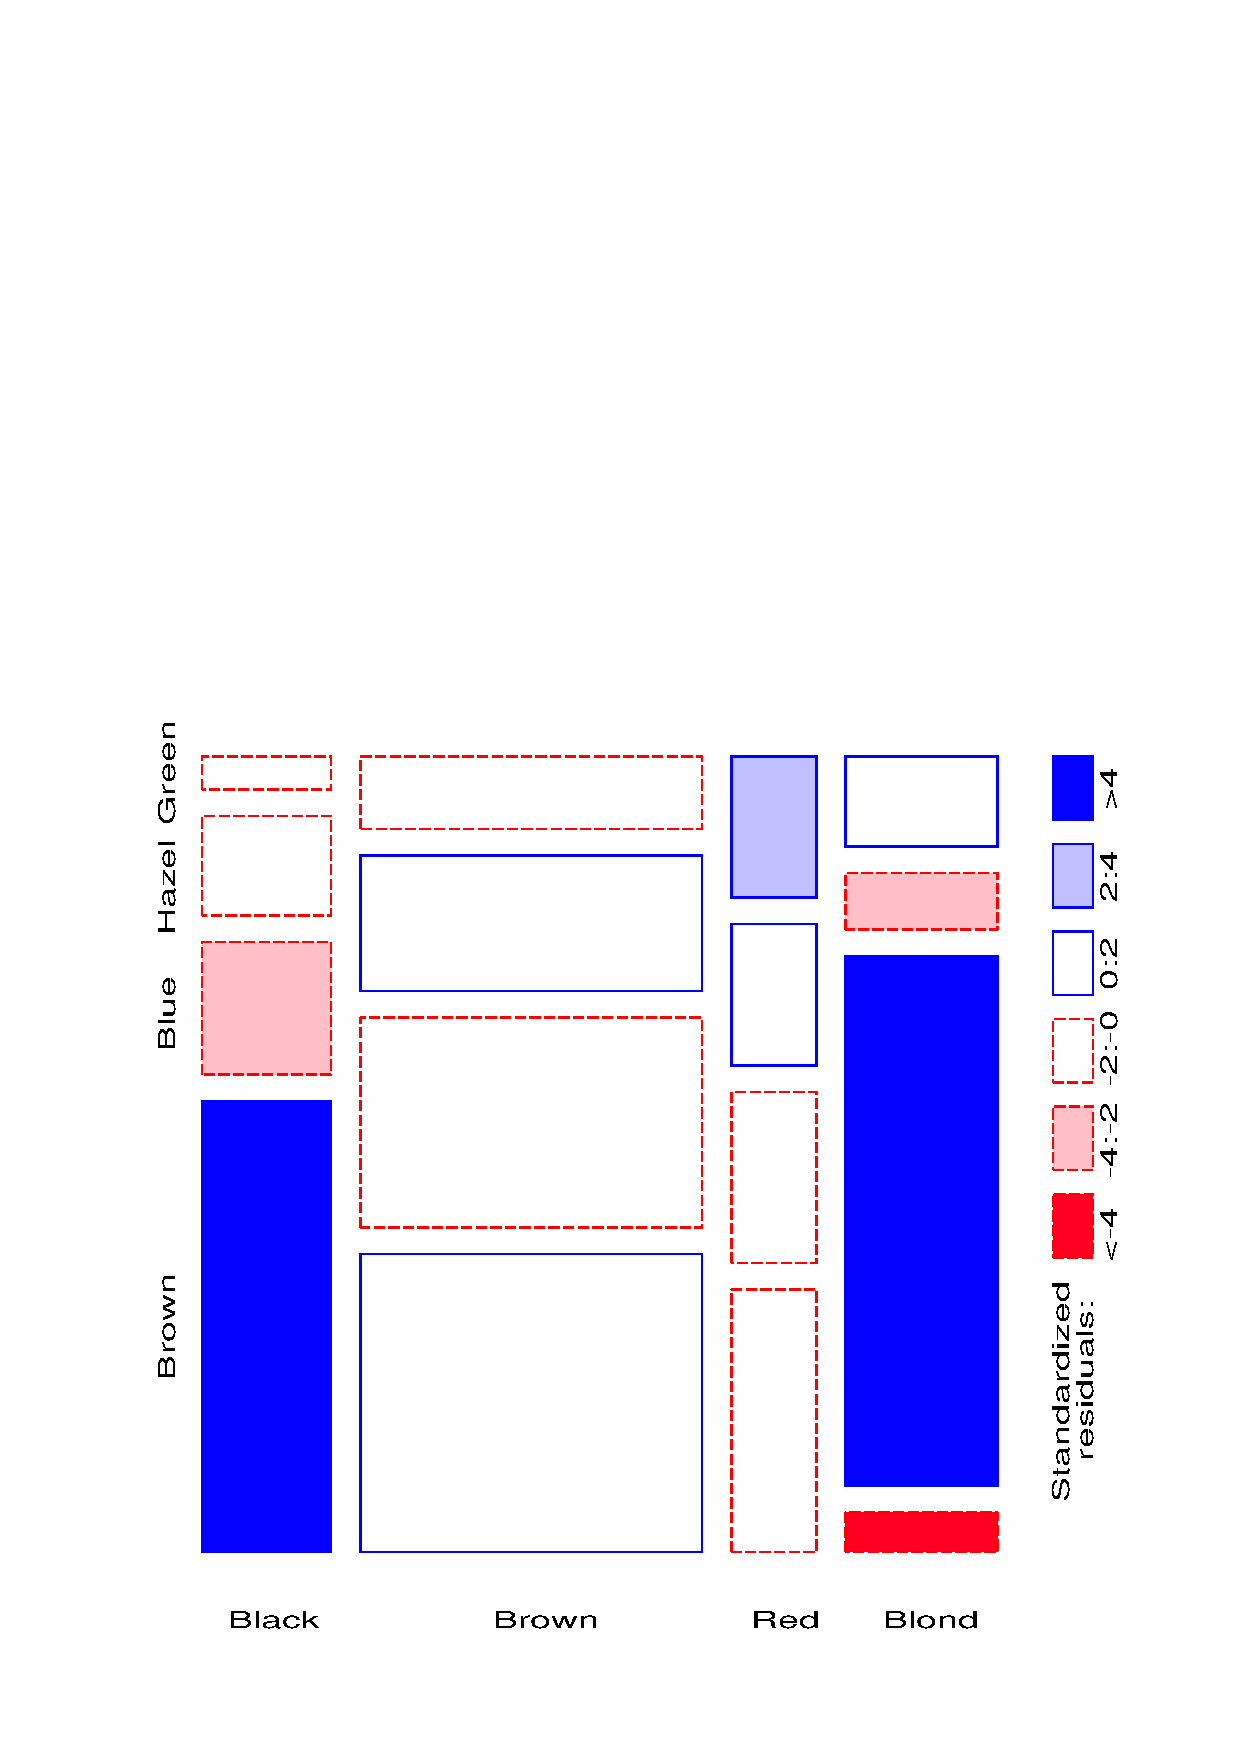
\includegraphics[scale=.6]{ch4/fig/mosaic33}
  \caption[Second step in the mosaic display]{Second step in the mosaic display.  Each rectangle for hair color is subdivided in proportion to the
  frequencies of eye color.}%
  \label{fig:mosaic33}
\end{figure}

\begin{itemize}
\item Again, the cells are shaded in relation to standardized
residuals, \(d_{ij} = (
n_{ij} - m_{ij}) / \sqrt { m_{ij} }\), 
from a model.  For a two-way table, the model is that Hair color and
Eye color are independent in the population from which this sample
was drawn.
\begin{verbatim} 
               Standardized Pearson residuals
               Brown     Blue    Hazel    Green

      Black     4.40    -3.07    -0.48    -1.95
      Brown     1.23    -1.95     1.35    -0.35
      Red      -0.07    -1.73     0.85     2.28
      Blond    -5.85     7.05    -2.23     0.61
\end{verbatim}
\item Thus, the two tiles shaded deep blue correspond to the two
cells, (Black, Brown) and (Blond, Blue), whose residuals are
greater than $+4$, indicating much greater frequency in those
cells than would be found if Hair color and Eye color were
independent.
The tile shaded deep red, (Blond, Brown)
corresponds to the largest residual = -5.85, indicating this combination
is extremely rare under the hypothesis of independence.
\item The overall Pearson \chisq{} statistic is just the
sum of squares of the residuals.
\end{itemize}
\end{Example}

\subsubsection{Shading levels}

The default shading patterns for the tiles are based on standardized
residuals which exceed the values 2 and 4 in absolute value.%
\footnote{In \Dset{}s with very large total frequency,
most models may fit poorly and have large residuals.
In such cases (e.g., \exref{ex:suicide1}) it is often useful to define
more shading levels to make finer distinctions.  For example,
in \exref{ex:suicide1} we use \pname{SHADE=\{2 4 8\};} to set
three levels of shading.}
Since the standardized residuals are approximately unit-normal $N(0,1)$
values,  this corresponds to highlighting cells whose
residuals are \emph{individually} significant at approximately
the .05 and .0001 level, respectively.
The purpose of highlighting cells, however, is not to provide tests
of significance, but rather to draw attention to the \emph{pattern}
of departures of the data from the assumed model.
In any case, 
the number and values of
these cutoffs can be easily set by the user using the \pname{SHADE}
parameter.

To provide some redundancy when color figures are reproduced in 
black and white, cells with positive residuals are outline with solid
(blue) lines, while cells with negative residuals are outlined with broken
(red) lines.
Cells whose absolute residuals are less than the smallest shading level
are unfilled.  For good-fitting models, it is sometimes useful to distinguish
between near-zero residuals and small, non-significant residuals.
In color figures, near-zero cells are outlined in solid black;
the threshold is determined by the \pname{FUZZ} parameter.

\subsubsection{Interpretation}

To interpret the association between Hair color and Eye color,
consider the pattern of positive (Blue) and negative (Red)
tiles in the mosaic display.  
We interpret positive values as showing cells whose observed frequency
is substantially greater than would be found under independence;
negative values indicate cells which occur less often than
under independence.

\ixe{Hair color and eye color|(}
This interpretation is enhanced by reordering the rows or columns
of the two-way table so that the residuals have an opposite
corner pattern of signs.  This usually helps us interpret any systematic
patterns of association in terms of the ordering of the row and column
categories.
Here, this is achieved by reordering the Eye colors as shown in
\figref{fig:mosaic34},  and we note that in this rearrangement
both hair colors and eye colors are ordered from dark to light.
(In general, the levels of a factor may be reordered by
arranging them according to their scores on the first (largest)
correspondence analysis dimension; see
\citep{Friendly:94a}).
The re-ordered residuals are:
\begin{verbatim} 
         Standardized Pearson residuals

          Brown    Hazel    Green     Blue

Black      4.40    -0.48    -1.95    -3.07
Brown      1.23     1.35    -0.35    -1.95
Red       -0.07     0.85     2.28    -1.73
Blond     -5.85    -2.23     0.61     7.05
\end{verbatim}
\begin{figure}[htb]
  \centering
  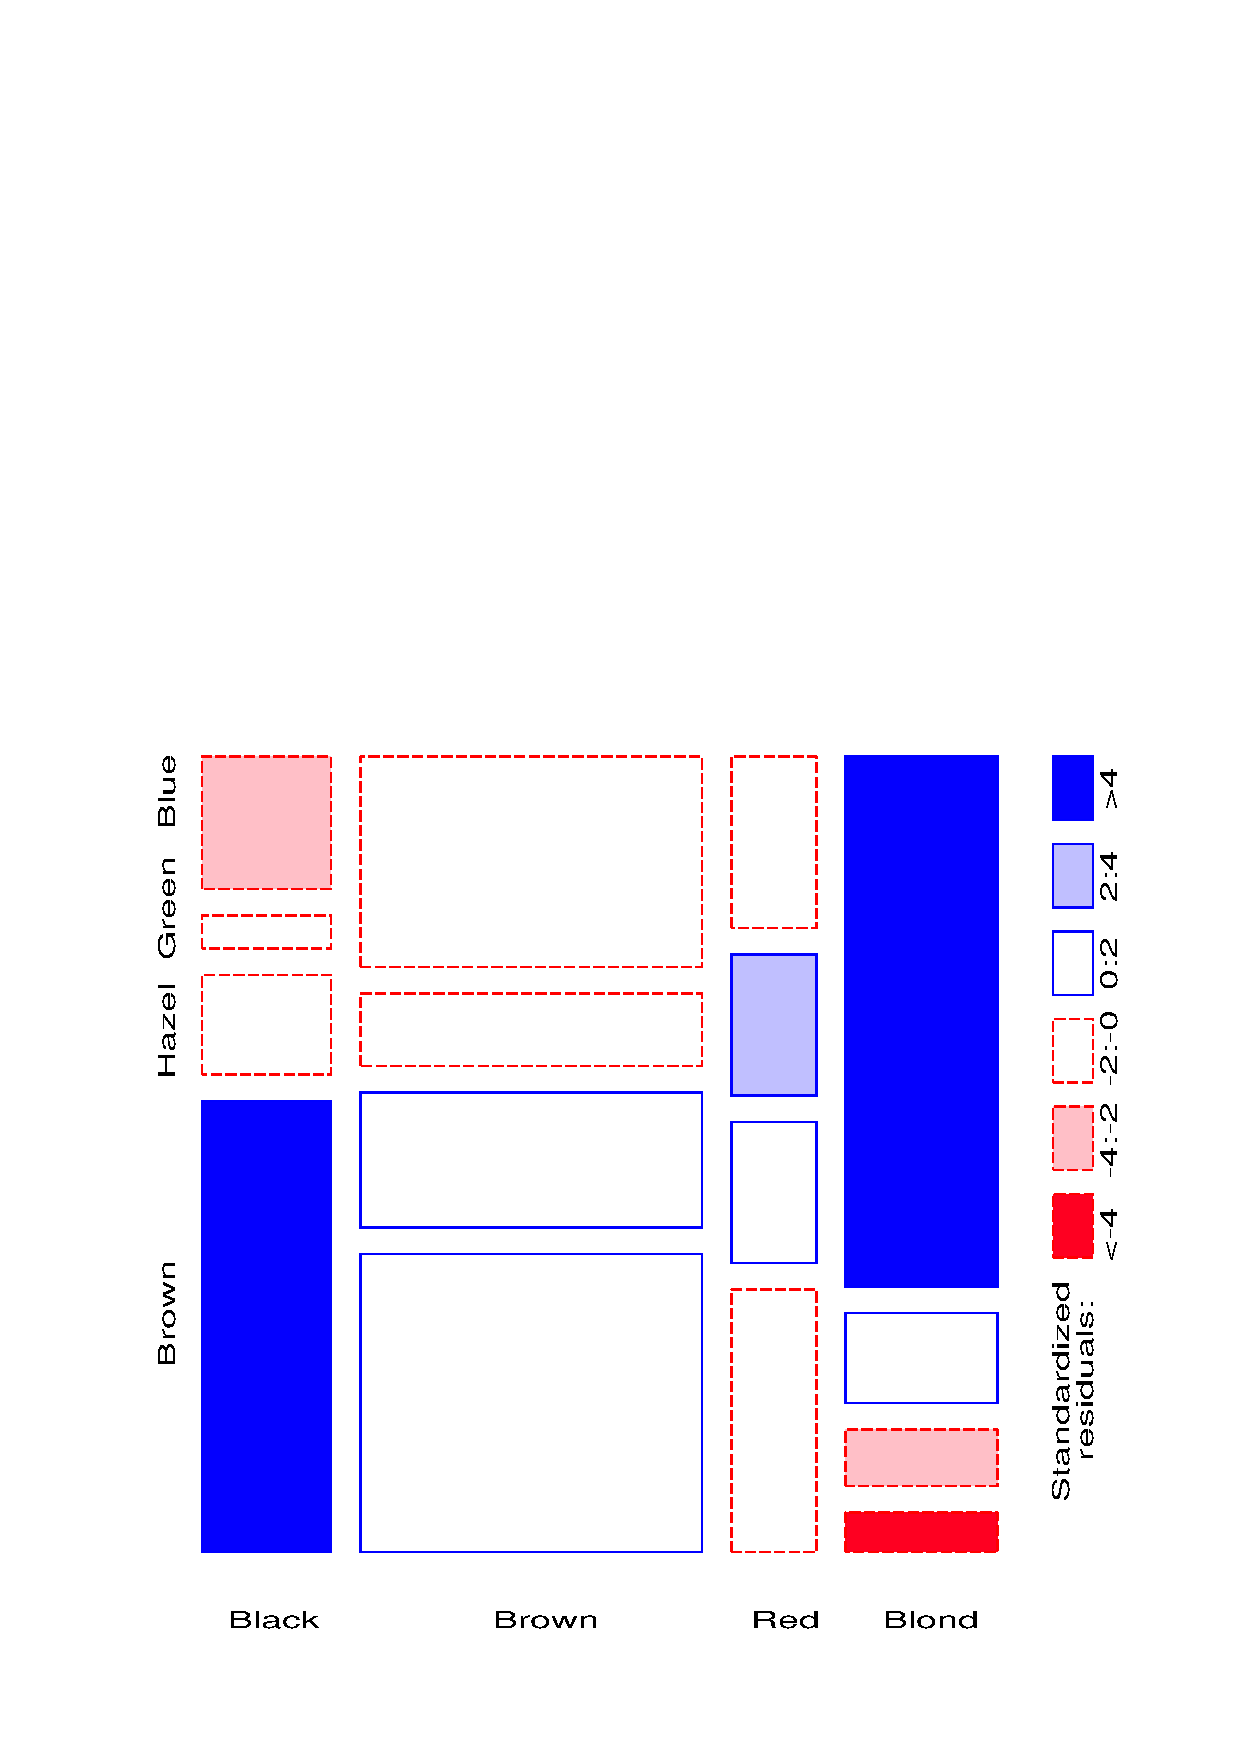
\includegraphics[scale=.6]{ch4/fig/mosaic34}
  \caption[Two-way mosaic, reordered]{Two-way mosaic,
  reordered.  Deviations from independence are shown by
  color and shading.  The two levels of shading density correspond to
  standardized deviations greater than 2 and 4 in absolute value.
  This form of the display generalizes readily to multi-way
  tables.}  \label{fig:mosaic34}
\end{figure}
Thus, the mosaic shows that the association between Hair and Eye color
is essentially that 
\begin{itemize*}
\item people with dark hair tend to have dark eyes,
\item those with light hair tend to have light eyes
\item people with red hair do not quite fit this pattern
\end{itemize*}
\ixe{Hair color and eye color|)}

\subsection{Software for mosaic displays}
Mosaic displays are implemented as a collection of modules
(the \sasprog{mosaics.sas}) written in \IML{},
which are used within a \PROC{IML} step,
as described in \macref{mac:mosaics}.  The program is designed so that
the frequency table, and its associated factor levels and variable names
may be entered directly using \IML{} statements,
or (using the \module{readtab}) may be input from a SAS \Dset\
of the form produced by \PROC{FREQ}.
Using the \sasprog{mosaics.sas} within a \PROC{IML} step is most
flexible, because you can use \IML{} statements and modules within
\texttt{mosaics.sas} to manipulate the frequency table (selecting
or reordering rows or columns), to specify structural zeros,
or to fit specialized models which cannot be fit by other means.

In addition, several SAS macros
are provided to simplify the use of \texttt{mosaics.sas}. 
The \macro{MOSAIC} (described in \macref{mac:mosaic})
may be used with any SAS \Dset\ in frequency
form (e.g., the output from \PROC{FREQ}).  It reads the data into
\IML{} and provides basic mosaic displays,
mosaics for externally-calculated residuals,
and partial mosaic displays (\secref{sec:mospart}).
The \macro{TABLE} (\macref{mac:table}) may be used to construct the frequency table, and
to collapse or recode variables.
The \macro{MOSMAT} (\macref{mac:mosmat})
provides mosaic matrices (\secref{sec:mosmat}),
an analog of the \scatmat{} for categorical data.

Two examples below illustrate the use of this software for basic mosaic
displays.
\exref{ex:soccer2} uses the \macro{MOSAIC},
while \exref{ex:victims}
uses \PROC{IML} statements to construct and manipulate the
frequency table.

\begin{table}[!hb]
\caption{Total goals scored in 380 games in the Premier
Football League, 1995/95 season}
\label{tab:soccer2}
\vspace{.1in}
\begin{center}
\begin{tabular}{l|rrrr rrrr}
\hline
Total goals      &  0  &  1  &  2  &  3  &  4  &  5  &  6  &  7  \\
\hline
Number of games  & 27  & 88  & 91  & 73  & 49  & 31  & 18  &  3  \\
  \hline
\end{tabular}
\end{center}
\end{table}

%%
% Table victims written by md2tex  1-29-1998
\begin{table}[htb]
 \caption{Repeat Victimization Data}
 \label{tab:victims}
 \begin{center}
  \begin{tabular}{|l|rrrrrrrr|}
   \hline
 & \multicolumn{8}{c|}{\bfseries\large First Victimization }\rule{0in}{2.5ex}\\
{\bfseries\large Second       } &          &       &       & Pick     & Personal &      & Household & Auto    \\
{\bfseries\large Victimization} & Rape     & Assault & Robbery & Pocket & Larceny & Burglary & Larceny & Theft   \\
   \hline
% f=        2 t=        1
Rape                   &            26 &            65 &            12 &             3 &            75 &            52 &            42 &             3 \\
Assault                &            50 &          2997 &           279 &           102 &          2628 &          1117 &          1251 &           221 \\
Robbery                &            11 &           238 &           197 &            40 &           413 &           191 &           206 &            51 \\
Pick Pocket            &             6 &            85 &            36 &            61 &           329 &           102 &           117 &            24 \\
Personal Larceny           &            82 &          2553 &           459 &           243 &         12137 &          2649 &          3757 &           678 \\
Burglary               &            39 &          1083 &           197 &           115 &          2658 &          3210 &          1962 &           301 \\
Household Larceny           &            48 &          1349 &           221 &           101 &          3689 &          1973 &          4646 &           367 \\
Auto Theft             &            11 &           216 &            47 &            38 &           687 &           301 &           391 &           269 \\
   \hline
  \end{tabular}
 \end{center}
\end{table}

